% Options for packages loaded elsewhere
\PassOptionsToPackage{unicode}{hyperref}
\PassOptionsToPackage{hyphens}{url}
\documentclass[
]{article}
\usepackage{xcolor}
\usepackage[margin=1in]{geometry}
\usepackage{amsmath,amssymb}
\setcounter{secnumdepth}{-\maxdimen} % remove section numbering
\usepackage{iftex}
\ifPDFTeX
  \usepackage[T1]{fontenc}
  \usepackage[utf8]{inputenc}
  \usepackage{textcomp} % provide euro and other symbols
\else % if luatex or xetex
  \usepackage{unicode-math} % this also loads fontspec
  \defaultfontfeatures{Scale=MatchLowercase}
  \defaultfontfeatures[\rmfamily]{Ligatures=TeX,Scale=1}
\fi
\usepackage{lmodern}
\ifPDFTeX\else
  % xetex/luatex font selection
\fi
% Use upquote if available, for straight quotes in verbatim environments
\IfFileExists{upquote.sty}{\usepackage{upquote}}{}
\IfFileExists{microtype.sty}{% use microtype if available
  \usepackage[]{microtype}
  \UseMicrotypeSet[protrusion]{basicmath} % disable protrusion for tt fonts
}{}
\makeatletter
\@ifundefined{KOMAClassName}{% if non-KOMA class
  \IfFileExists{parskip.sty}{%
    \usepackage{parskip}
  }{% else
    \setlength{\parindent}{0pt}
    \setlength{\parskip}{6pt plus 2pt minus 1pt}}
}{% if KOMA class
  \KOMAoptions{parskip=half}}
\makeatother
\usepackage{graphicx}
\makeatletter
\newsavebox\pandoc@box
\newcommand*\pandocbounded[1]{% scales image to fit in text height/width
  \sbox\pandoc@box{#1}%
  \Gscale@div\@tempa{\textheight}{\dimexpr\ht\pandoc@box+\dp\pandoc@box\relax}%
  \Gscale@div\@tempb{\linewidth}{\wd\pandoc@box}%
  \ifdim\@tempb\p@<\@tempa\p@\let\@tempa\@tempb\fi% select the smaller of both
  \ifdim\@tempa\p@<\p@\scalebox{\@tempa}{\usebox\pandoc@box}%
  \else\usebox{\pandoc@box}%
  \fi%
}
% Set default figure placement to htbp
\def\fps@figure{htbp}
\makeatother
\setlength{\emergencystretch}{3em} % prevent overfull lines
\providecommand{\tightlist}{%
  \setlength{\itemsep}{0pt}\setlength{\parskip}{0pt}}
\usepackage{titlesec}
\titleformat{\section}{\centering\normalfont\Large\bfseries}{\thesection}{1em}{}
\titleformat{\subsection}{\centering\normalfont\large\bfseries}{\thesubsection}{1em}{}
\titleformat{\subsubsection}{\centering\normalfont\normalsize\bfseries}{\thesubsubsection}{1em}{}
\usepackage{booktabs}
\usepackage{longtable}
\usepackage{array}
\usepackage{multirow}
\usepackage{wrapfig}
\usepackage{float}
\usepackage{colortbl}
\usepackage{pdflscape}
\usepackage{tabu}
\usepackage{threeparttable}
\usepackage{threeparttablex}
\usepackage[normalem]{ulem}
\usepackage{makecell}
\usepackage{xcolor}
\usepackage{bookmark}
\IfFileExists{xurl.sty}{\usepackage{xurl}}{} % add URL line breaks if available
\urlstyle{same}
\hypersetup{
  pdftitle={Prueba},
  pdfauthor={Sofia},
  hidelinks,
  pdfcreator={LaTeX via pandoc}}

\title{Prueba}
\author{Sofia}
\date{2025-03-04}

\begin{document}
\maketitle

\section{Analisis Bivariante}\label{analisis-bivariante}

\begin{table}[!h]
\centering
\caption{\label{tab:tabla1 }Desempeño En Comparación al Nivel Educativo de los Padres}
\centering
\begin{tabular}[t]{lrrrrr}
\toprule
  & {}[9,32) & {}[32,55) & {}[55,78) & {}[78,100] & Sum\\
\midrule
\cellcolor{gray!10}{associate's degree} & \cellcolor{gray!10}{1} & \cellcolor{gray!10}{37} & \cellcolor{gray!10}{121} & \cellcolor{gray!10}{63} & \cellcolor{gray!10}{222}\\
bachelor's degree & 0 & 12 & 68 & 38 & 118\\
\cellcolor{gray!10}{high school} & \cellcolor{gray!10}{4} & \cellcolor{gray!10}{53} & \cellcolor{gray!10}{111} & \cellcolor{gray!10}{28} & \cellcolor{gray!10}{196}\\
master's degree & 0 & 7 & 28 & 24 & 59\\
\cellcolor{gray!10}{some college} & \cellcolor{gray!10}{4} & \cellcolor{gray!10}{29} & \cellcolor{gray!10}{135} & \cellcolor{gray!10}{58} & \cellcolor{gray!10}{226}\\
\addlinespace
some high school & 5 & 39 & 97 & 38 & 179\\
\cellcolor{gray!10}{Sum} & \cellcolor{gray!10}{14} & \cellcolor{gray!10}{177} & \cellcolor{gray!10}{560} & \cellcolor{gray!10}{249} & \cellcolor{gray!10}{1000}\\
\bottomrule
\end{tabular}
\end{table}

\pandocbounded{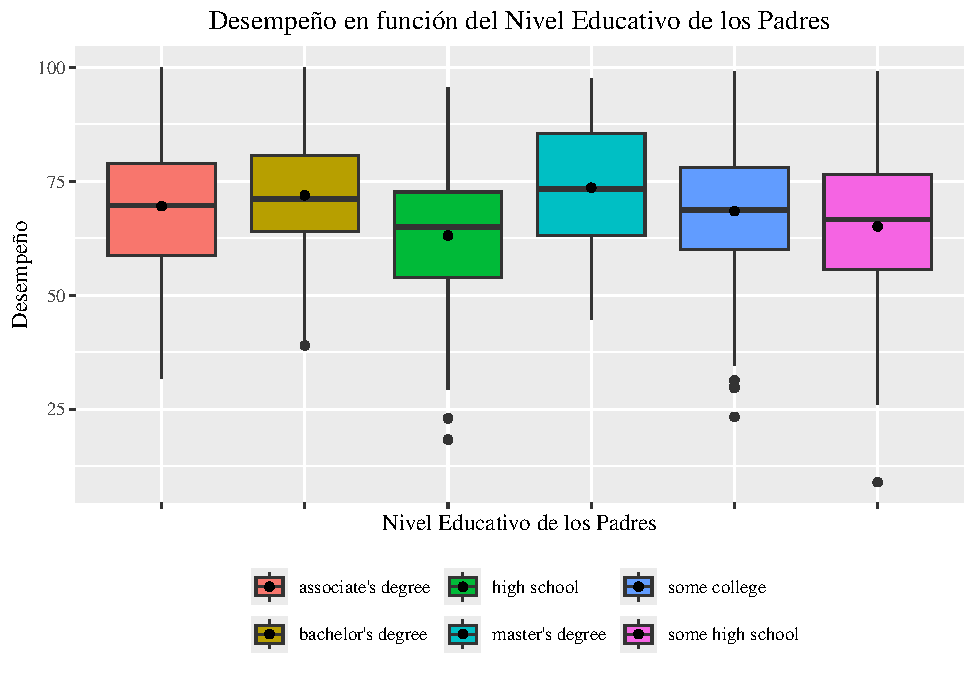
\includegraphics[keepaspectratio]{prueva1_files/figure-latex/grafico1-1.pdf}}

\begin{table}[!h]
\centering
\caption{\label{tab:tabla2 }Desempeño En Comparación al Tipo de Almuerzo}
\centering
\begin{tabular}[t]{lrrrrr}
\toprule
  & {}[9,32) & {}[32,55) & {}[55,78) & {}[78,100] & Sum\\
\midrule
\cellcolor{gray!10}{free/reduced} & \cellcolor{gray!10}{11} & \cellcolor{gray!10}{96} & \cellcolor{gray!10}{196} & \cellcolor{gray!10}{52} & \cellcolor{gray!10}{355}\\
standard & 3 & 81 & 364 & 197 & 645\\
\cellcolor{gray!10}{Sum} & \cellcolor{gray!10}{14} & \cellcolor{gray!10}{177} & \cellcolor{gray!10}{560} & \cellcolor{gray!10}{249} & \cellcolor{gray!10}{1000}\\
\bottomrule
\end{tabular}
\end{table}

\pandocbounded{\includegraphics[keepaspectratio]{prueva1_files/figure-latex/grafico2-1.pdf}}

\pandocbounded{\includegraphics[keepaspectratio]{prueva1_files/figure-latex/grafico3-1.pdf}}

\end{document}
